\documentclass[tikz]{standalone}

\usepackage{tkz-tab}
\usepackage{amsmath, amssymb}
\usepackage[fontsize=14pt]{fontsize}

\begin{document}
    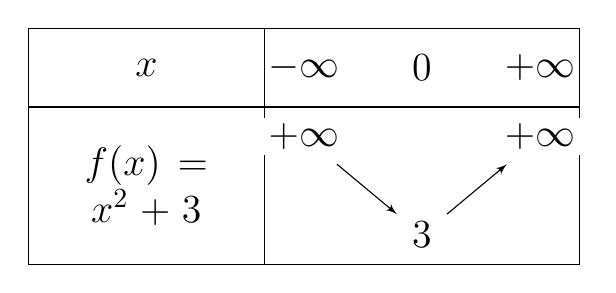
\begin{tikzpicture}
        \tkzTabInit[lgt=3, espcl=1.5]
        {$x$ / 1 , $f(x) = x^2 + 3$ / 2}
        {$-\infty$, $0$, $+\infty$}
        %\tkzTabLine
        %{ , , }
        \tkzTabVar
        { +/$+\infty$, -/$3$, +/$+\infty$}
    \end{tikzpicture}

    \begin{tikzpicture}
        \draw[->] (-3, 0) -- (3, 0) node[right] {$x$};
      \draw[->] (0, -1) -- (0, 8) node[above] {$y$};
      \draw[scale=1, domain=-2:2, smooth, variable=\x, red] plot ({\x}, {\x*\x + 3})
        node[right, black, above] {$y = x^2 + 3$};
      %\draw[scale=0.5, domain=-3:3, smooth, variable=\y, red]  plot ({\y*\y}, {\y});
    \end{tikzpicture}

    \begin{tikzpicture}
        \draw[->] (-4, 0) -- (4, 0) node[right] {$x$};
        \draw[->] (0, -4) -- (0, 4) node[above] {$y$};
        \draw[scale=1, domain=-4:-0.3, smooth, variable=\x, red] plot ({\x}, {1 / \x})
        node[below left, black] {$y = \dfrac{1}{x}$};
        \draw[scale=1, domain=0.3:4, smooth, variable=\x, red] plot ({\x}, {1 / \x})
        node[above, black] {$y = \dfrac{1}{x}$};
      %\draw[scale=0.5, domain=-3:3, smooth, variable=\y, red]  plot ({\y*\y}, {\y});
    \end{tikzpicture}
\end{document}